\section{Perturbation of the Orbital Elements} \label{sec:PerturbationMethod}
In the previous chapter we've solved the 2-body problem in Newtonian mechanics and the solution involves six initial conditions, e.g. components of the initial relative position and initial relative velocity, that we have replaced by the six orbital elements, which will be denoted as $\vartheta ^a = \{ a,e, \iota, \Omega, \omega, l_0 \}$. Hence, the solution of the Newtonian 2-body problem is formally expressed by the functions
\begin{subequations} \label{eq:2BodyNewtonianSolution}
\begin{align}
\textbf{x} (t) &= \textbf{x}_N (t, \vartheta^a) \\
\dot{\textbf{x}} (t) &= \dot{\textbf{x}}_N (t, \vartheta^a)
\end{align}
\end{subequations}
where the Newtonian vectors satisfy the  equations of motion
\begin{subequations}
\begin{align}
\dot{\textbf{x}}_N &= \frac{d \textbf{x}_N}{dt} \\
\ddot{\textbf{x}}_N &= \frac{d \dot{\textbf{x}}_N}{dt} = - \frac{GM}{r_N^3} \textbf{x}_N \, ,
\end{align}
\end{subequations}
where $M=m_1 + m_2$ is the total mass of the system.

In this chapter, we will  introduce a perturbing force per unit mass $\delta \textbf{A}= \frac{\delta \textbf{F}}{\mu}$ which will account for small external influences on the 2-body system.  Using the time dependent basis $(\textbf{n}, \boldsymbol{\lambda}, \textbf{k})$, introduced in (\ref{eq:2BodyTimeDependentBasis}), we write the equation of motion, including the perturbing force, as
\begin{equation}
\ddot{\textbf{x}} = -\frac{GM}{r^2} \textbf{n} + \delta \textbf{A} ,
\end{equation}
where $\textbf{n} = \frac{\textbf{x}}{r}$ is the unit vector in the relative radial direction and the components of $\delta \textbf{A}$ are written as
\begin{equation}
\delta \textbf{A} = \mathcal{S} \textbf{n} + \mathcal{T} \boldsymbol{\lambda} + \mathcal{W} \textbf{k} \label{eq:PerturbingForce}
\end{equation}
with the components
\begin{equation} 
\begin{cases}
\mathcal{S} &= \delta \textbf{A} \cdot \textbf{n} \\
\mathcal{T} &=  \delta \textbf{A}  \cdot \boldsymbol{\lambda} \\
\mathcal{W} &=  \delta \textbf{A}  \cdot \textbf{k} .
\end{cases} \label{eq:PerturbingForceComponents}
\end{equation}

We will assume that $ \delta \textbf{A} $ is small compared with the Newtonian gravitational force and therefore, the description in the previous chapter is approximately correct. The effect of the perturbing force will be that the orbit is no longer a fixed conic in space. Hence, the approach that we will use to obtain the perturbed solution is to use the Newtonian solution (\ref{eq:2BodyNewtonianSolution}) considering that the orbital elements are now functions of time, $\vartheta^a = \vartheta^a (t)$.  
The perturbed solution will have the form 
\begin{subequations} 
\begin{align}
\textbf{x} (t) &= \textbf{x}_N (t, \vartheta^a (t)) \\
\dot{\textbf{x}} (t) &= \dot{\textbf{x}}_N (t, \vartheta^a (t)) .
\end{align}
\end{subequations}

%
% Finding the osculating elements. Option 1
%from which we obtain
%\begin{subequations} 
%\begin{align}
%\frac{d\textbf{r}}{dt} &= \frac{\partial \textbf{r}_N}{\partial t} + \sum_a \frac{\partial \textbf{r}_N}{\partial \vartheta ^a} \frac{d\vartheta^a}{dt} \\
%\frac{d \dot{\textbf{r}}}{dt} &= \frac{\partial \dot{\textbf{r}}_N}{\partial t} + \sum_a \frac{\partial \dot{\textbf{r}}_N}{\partial \vartheta ^a} \frac{d\vartheta^a}{dt} .
%\end{align}
%\end{subequations}
%
%Comparison with the perturbed equation of motion gives the conditions
%\begin{subequations} 
%\begin{align}
%\sum_a \frac{\partial \textbf{r}_N}{\partial \vartheta ^a} \frac{d\vartheta^a}{dt} &= 0 \\
%\sum_a \frac{\partial \dot{\textbf{r}}_N}{\partial \vartheta ^a} \frac{d\vartheta^a}{dt} &= \textbf{F} ,
%\end{align}
%\end{subequations}
%which can be formally solved to obtain the orbital elements as functions of time. However, we will follow another approach to obtain the differential equations defining the orbital elements. 
%

In order to obtain the differential equations defining the orbital elements, we note that the angular momentum per unit mass, $\boldsymbol{\ell} = \ell \textbf{k} = \textbf{x} \times \dot{\textbf{x}}$, is now a vector that changes with time,
\begin{equation}
\frac{d\boldsymbol{ \ell}}{dt} = \textbf{x} \times \delta \textbf{A}.
\end{equation}

Using the perturbation in equation (\ref{eq:PerturbingForce}), we get
\begin{equation}
\frac{d\boldsymbol{ \ell}}{dt} = - r\mathcal{W} \boldsymbol{\lambda}  + r\mathcal{T} \textbf{k}.
\end{equation}
from which we conclude that
\begin{subequations}
\begin{align}
\frac{d\ell}{dt} &= r \mathcal{T}\\
\ell \frac{d \textbf{k}}{dt} &= - r\mathcal{W} \boldsymbol{\lambda}.
\end{align}
\end{subequations}

\begin{exercise}[Laplace-Runge-Lenz variation in time]
\textbf{Laplace-Runge-Lenz variation in time}

Consider the eccentricity vector given in equations (\ref{eq:2BodyLaplaceVector}) and (\ref{eq:2BodyLaplaceVector2}),
\begin{align}
\textbf{e} = &\frac{\dot{\textbf{x}}\times \boldsymbol{\ell}}{GM} - \textbf{n} = e \left[ \cos f \textbf{n} - \sin f \boldsymbol{\lambda} \right]. 
\end{align}
Show that its time derivative is 
\begin{align}
\frac{d \textbf{e}}{dt} = &\frac{1}{GM}\left[ \delta \textbf{A} \times \boldsymbol{\ell} + \dot{\textbf{x}} \times (\textbf{x} \times \delta \textbf{A}) \right] \notag \\
= &\frac{1}{GM}\left[ 2\ell \mathcal{T} \textbf{n} - (\ell \mathcal{S} + r \dot{r} \mathcal{T}) \boldsymbol{\lambda} - r\dot{r} \mathcal{W} \textbf{k} \right].
\end{align}
Also show that this equation implies the relations
\begin{equation}
\frac{de}{dt} = \frac{1}{GM}\left[ \ell \sin f \mathcal{S} + \left( 2 \ell \cos f + r \dot{r} \sin f \right)\mathcal{T} \right]
\end{equation}
and
\begin{align}
\frac{d}{dt}\left( \frac{\textbf{e}}{e}\right) = &\frac{1}{GMe}\left[ -\ell \cos f \mathcal{S} + \left( 2 \ell \sin f - r \dot{r} \cos f \right)\mathcal{T} \right] \left[ \cos f \textbf{n} + \sin f \boldsymbol{\lambda}\right] - \frac{r \dot{r} \mathcal{W}}{GMe} \textbf{k}.
\end{align}
\end{exercise}

\subsection{Osculating Elements}
Now we are ready to obtain the time dependence of the orbital elements. Differentiating equations (\ref{eq:2BodyOrbitalElements}) and using the above results, we obtain the differential equations known as \textit{osculating elements} or as \textit{Lagrange's planetary equations},
\begin{subequations}\label{eq:OsculatingOrbitalElements}
\begin{align}
\frac{da}{dt} &= 2\sqrt{\frac{a^3}{GM (1-e^2)}} \left[ e \sin f \mathcal{S} + (1+e\cos f) \mathcal{T} \right] \\
\frac{de}{dt} &= \sqrt{\frac{p}{GM}} \left[ \sin f \mathcal{S} + \frac{2\cos f + e \left( 1 + \cos^2 f \right) }{1 + e\cos f} \mathcal{T} \right] \\
\frac{d \iota}{dt} &= \sqrt{\frac{p}{GM}} \frac{\cos (f+\omega)}{1+e\cos f} \mathcal{W} \\
\frac{d \Omega}{dt} &= \sqrt{\frac{p}{GM}} \frac{\sin (f+\omega)}{(1+e\cos f)\sin \iota } \mathcal{W} \\
\frac{d\omega}{dt} &=\frac{1}{e}\sqrt{\frac{p}{GM}} \left[ -\cos f \mathcal{S} + \frac{2+e\cos f}{1 + e \cos f} \sin f \mathcal{T} - e  \frac{\sin (f + \omega)}{1 + e \cos f} \cot \iota \mathcal{W} \right] \\
\frac{dl_0}{dt} &= -\sqrt{1-e^2} \left[ \frac{d\omega}{dt} + \cos \iota \frac{d\Omega}{dt} - \frac{2p}{na^2 (1+e \cos f)} \mathcal{T} \right] .
\end{align}
\end{subequations}

We also include into this set the differential equation for the semi-latus rectum,
\begin{equation}
\frac{dp}{dt} = 2 \sqrt{\frac{p}{GM}} \frac{\mathcal{T}}{1+e\cos f} .
\end{equation}
%\begin{equation}
%\frac{dp}{dt} = \frac{2}{n} \frac{(1-e^2)^{3/2}}{1+e\cos f} \mathcal{T}.
%\end{equation}

From the relation
\begin{equation}
 \cos f = \frac{\textbf{n} \cdot \textbf{e}}{e}
 \end{equation} 
it is possible to obtain, after differentiation, the time evolution equation for the true anomaly,
 \begin{equation}
\frac{df}{dt} = \sqrt{\frac{GM}{p^3}} \left( 1 + e \cos f \right)^2 \left[ 1 + \frac{1}{e}\sqrt{\frac{p}{GM}} \left( \frac{\cos f}{(1+e \cos f) ^2} \mathcal{S} - \frac{2+e\cos f}{(1 + e\cos f)^3} \sin f \mathcal{T} \right) \right]. \label{eq:TrueAnomalyOsculatingEquation}
 \end{equation} 
 
Similarly, the time variation of the eccentric anomaly is obtained from Kepler's equation (\ref{eq:2BodyKeplerEquation}),
 \begin{equation}
\frac{dE}{dt} =  \frac{na}{r} - \frac{r}{a \sqrt{1-e^2}} \left[ \frac{d \omega }{dt} + \cos \iota \frac{d \Omega}{dt} + \frac{\sin f}{1 - e^2} \frac{de}{dt}  \right] .
 \end{equation}

\subsection{Secular Changes of the Orbital Elements}

The orbital elements may present periodic and non-periodic changes. The periodic contributions are not interesting because they average to zero after some revolutions. On the other hand, the changes in the orbital elements that doesn't average but accumulate over time are called \textit{secular changes} and are important because, after some time interval, they can produce a large departure from the initial unperturbed orbit. In order to obtain the secular changes in the orbital elements $\vartheta^a$, we integrate over one period of the orbit,
\begin{equation}
\Delta \vartheta^a = \int_0 ^T \frac{d\vartheta^a}{dt} dt. \label{eq:OsculatingSecularint}
\end{equation}

The time integration over one period can be replaced by an integration with the true anomaly using (\ref{eq:TrueAnomalyOsculatingEquation}) to change  variables,
\begin{equation}
\Delta \vartheta^a = \int_0 ^{2 \pi} \frac{d\vartheta^a}{df} df.\label{eq:OsculatingSecularinf}
\end{equation}  

Assuming that both the perturbing force and the changes in the orbital elements are small, the first order approximation of the osculating elements as function of the true anomaly gives the equation
%\begin{subequations}\label{eq:OsculatingOrbitalElementsinf}
%\begin{align}
%\frac{da}{df} &= \frac{2(1-e^2)}{n} \left[ \frac{e \sin f }{(1+e \cos f)^2}\mathcal{R} + \frac{1}{1+e\cos f} \mathcal{T} \right] \\
%\frac{de}{df} &= \frac{(1-e^2)^2}{n^2a} \left[ \frac{\sin f}{(1+e \cos f)^2} \mathcal{R} + \frac{2\cos f + e \left( 1 + \cos^2 f \right) }{(1 + e\cos f)^3} \mathcal{T} \right] \\
%\frac{d \iota}{df} &= \frac{(1-e^2)^2}{n^2 a} \frac{\cos (f+\omega)}{(1+e\cos f)^3} \mathcal{W} \\
%\frac{d \Omega}{df} &= \frac{(1-e^2)^2}{n^2 a}  \frac{\sin (f+\omega)}{(1+e\cos f)^3 \sin \iota } \mathcal{W} \\
%\frac{d\omega}{df} &=\frac{(1-e^2)^2}{n^2 a e}  \left[ - \frac{\cos f}{(1+e\cos f)^2} \mathcal{R} + \frac{2+e\cos f}{(1 + e \cos f)^3} \sin f \mathcal{T} - e  \frac{\sin (f + \omega)}{(1 + e \cos f)^3} \cot \iota \mathcal{W} \right] \\
%\frac{dl_0}{df} &= -\sqrt{1-e^2} \left( \frac{d\omega}{df} + \cos \iota \frac{d\Omega}{df} \right) + \frac{2 (1-e^2)^3}{n^2 a (1+e \cos f)^3} \mathcal{T}  ,
%\end{align}
%\end{subequations}
\begin{subequations}\label{eq:OsculatingOrbitalElementsinf}
\begin{align}
\frac{da}{df} &= \frac{2p^3}{GM(1-e^2)^2} \left[ \frac{e \sin f }{(1+e \cos f)^2}\mathcal{S} + \frac{1}{1+e\cos f} \mathcal{T} \right] \\
\frac{de}{df} &= \frac{p^2}{GM} \left[ \frac{\sin f}{(1+e \cos f)^2} \mathcal{S} + \frac{2\cos f + e \left( 1 + \cos^2 f \right) }{(1 + e\cos f)^3} \mathcal{T} \right] \\
\frac{d \iota}{df} &= \frac{p^2}{GM} \frac{\cos (f+\omega)}{(1+e\cos f)^3} \mathcal{W} \\
\frac{d \Omega}{df} &= \frac{p^2}{GM} \frac{\sin (f+\omega)}{(1+e\cos f)^3 \sin \iota } \mathcal{W} \\
\frac{d\omega}{df} &=\frac{p^2}{GMe}  \left[ - \frac{\cos f}{(1+e\cos f)^2} \mathcal{S} + \frac{2+e\cos f}{(1 + e \cos f)^3} \sin f \mathcal{T} - e  \frac{\sin (f + \omega)}{(1 + e \cos f)^3} \cot \iota \mathcal{W} \right] \\
\frac{dl_0}{df} &= -\sqrt{1-e^2} \left( \frac{d\omega}{df} + \cos \iota \frac{d\Omega}{df} \right) + \frac{2 (1-e^2)^3}{n^2 a (1+e \cos f)^3} \mathcal{T}  ,
\end{align}
\end{subequations}
together with a similar equation for the semi-latus rectum,
\begin{equation}
\frac{dp}{df} = \frac{2p^3}{GM} \frac{1}{(1+e\cos f)^3} \mathcal{T} .
\end{equation}
%\begin{equation}
%\frac{dp}{df} = \frac{2}{n^2} \frac{(1-e^2)^3}{(1+e\cos f)^3} %\mathcal{T} .
%\end{equation}

%%%
% Osculating Elements using the eccentric anomaly
%It is also usual to use the eccentric anomaly to perform the integration over one orbit, 
%\begin{equation}
%\Delta \vartheta^a = \int_0 ^{2 \pi} \frac{d\vartheta^a}{dE} dE.
%\end{equation}

%\begin{exercise}[Osculating Elements in Terms of the Eccentric Anomaly]
%\textbf{Osculating Elements in Terms of the Eccentric Anomaly}

%Use equations (\ref{eq:2BodyEandfRelations2}), (\ref{eq:2BodyEandfDerivatives}) and (\ref{eq:2BodyPositionwithE}) to obtain the osculating elements in terms of the eccentric anomaly,
%\begin{subequations}\label{eq:OsculatingOrbitalElementsinE}
%\small
%\begin{align}
%\frac{da}{dE} = &\frac{1}{n\sqrt{1-e^2}} \left[ e \sqrt{1-e^2} \sin E \mathcal{R} + \mathcal{T} \right] \\
%\frac{de}{dE} = &\frac{1-e^2}{n^2 a} \left[ \sin E \mathcal{R} + \frac{2\cos E - e \left( 1 + \cos^2 E \right) }{\sqrt{1-e^2}} \mathcal{T} \right] \\
%\frac{d \iota}{dE} = &\frac{1-e\cos E}{n^2 a \sqrt{1-e^2}} \left[ (\cos E - e) \cos \omega - \sqrt{1-e^2} \sin E \sin \omega  \right] \mathcal{W} \\
%\frac{d \Omega}{dE} = &\frac{1-e\cos E}{n^2 a \sqrt{1-e^2} \sin \iota}  \left[ \sqrt{1-e^2} \sin E \cos \omega + (\cos E - e) \sin \omega  \right] \mathcal{W} \\
%\frac{d\omega}{dE} =&\frac{1}{n^2 a e}  \left[ -  \sqrt{1-e^2} (\cos E - e) \mathcal{R} + \sin E (2 - e \cos E - e^2) \mathcal{T} \right. \notag \\
%& \left. \hspace{0.2cm} - \frac{e (1 - e\cos E)\left( \sqrt{1-e^2} \sin E \cos \omega + (\cos E - e) \sin \omega \right)}{(1 -e^2)^3} \cot \iota   \mathcal{W} \right] \\
%\frac{dl_0}{dE} = &-\sqrt{1-e^2} \left[ \frac{d\omega}{dE} + \cos \iota \frac{d\Omega}{dE}  + \frac{2 (1-e \cos E)^2}{n^2 a} \mathcal{T} \right].
%\end{align}
%\end{subequations}
%Also obtain the corresponding equation for the semi-latus rectum,
%\begin{equation}
%\frac{dp}{dE} = \frac{2 \sqrt{1-e^2}}{n^2} (1- e \cos E)^2 \mathcal{T} .
%\end{equation}
%\end{exercise}

%%%%

\section{Examples}\label{sec:Examples}

In order to illustrate the perturbation theory treatment, we will present two of the most important examples: the precession of the orbit of Mercury under the influence of another planet and the Kozai-Lidov effect on the orbit of an asteroid. Both examples consider the gravitational field of a third body as the perturbing force.


\begin{figure}[h]
\centering
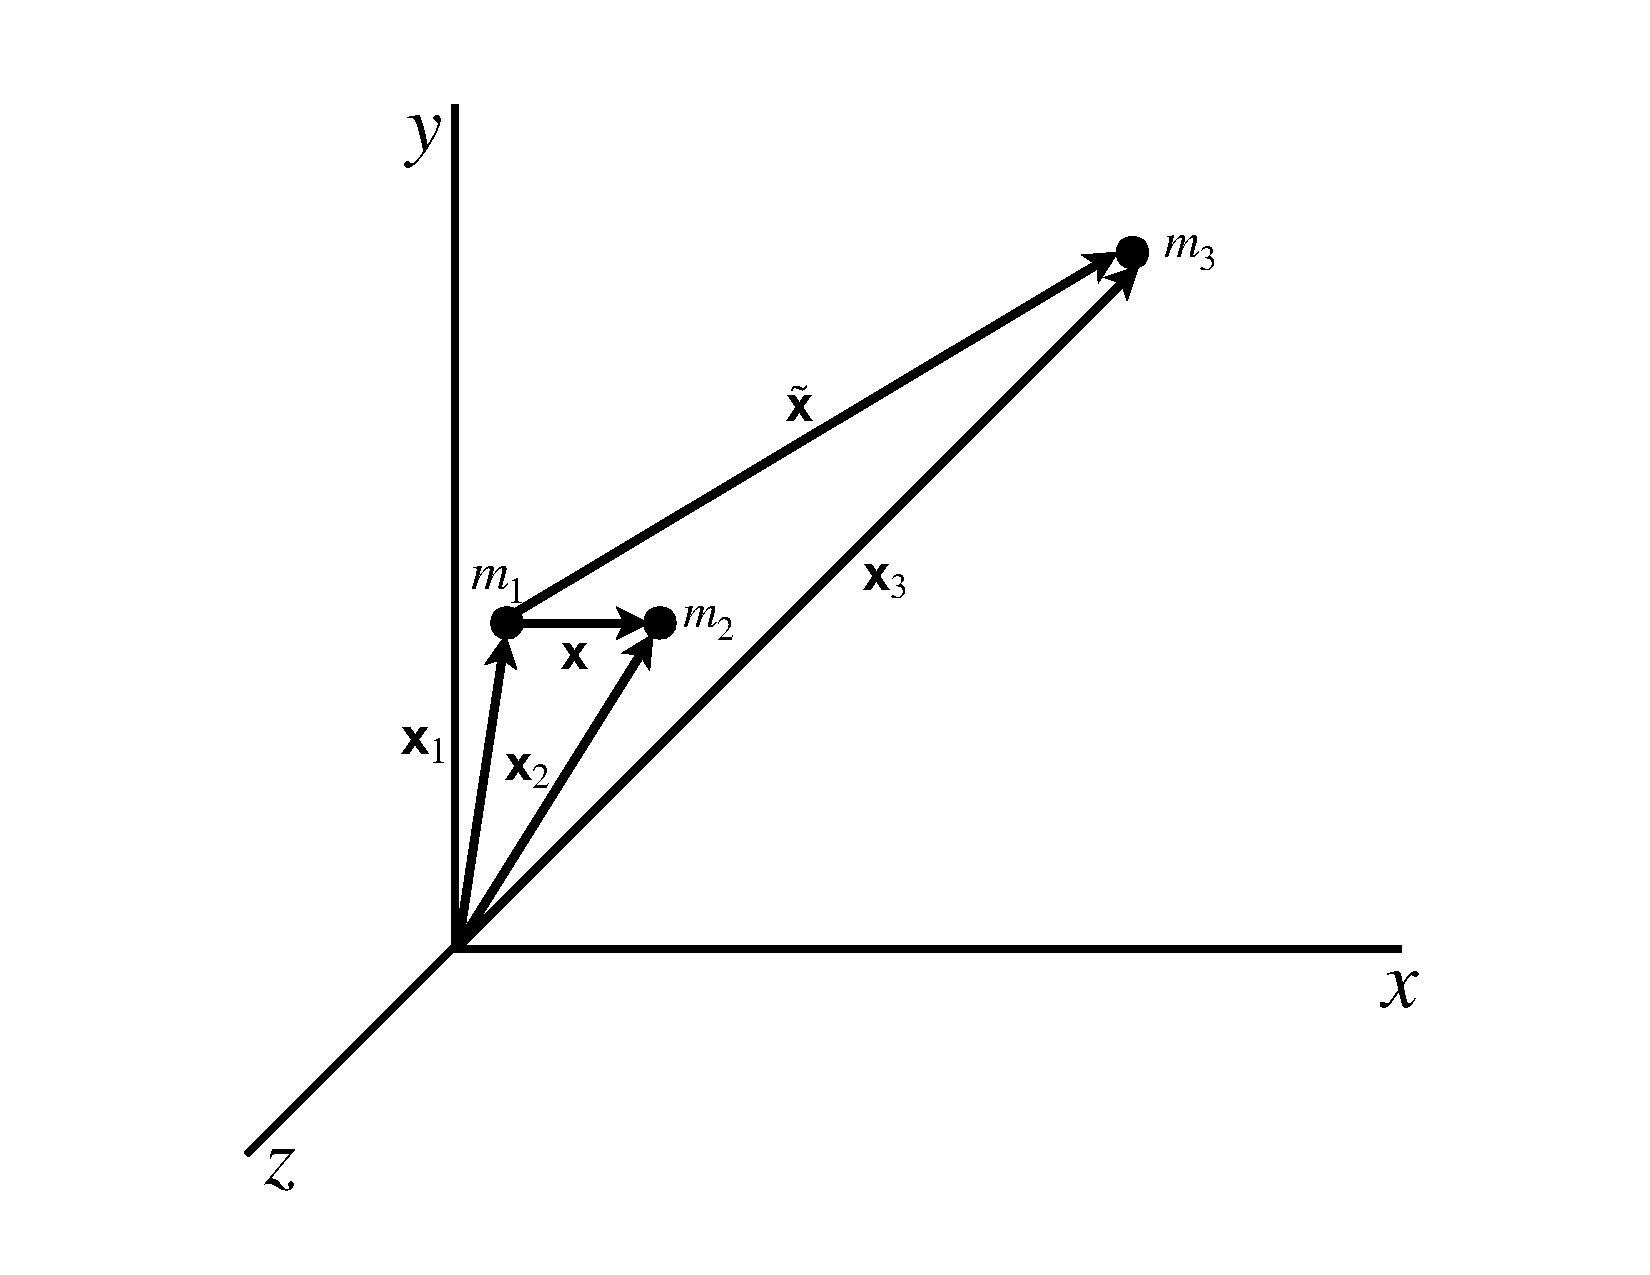
\includegraphics[width=0.6\linewidth]{3Body}
\caption[3-Body System.]
{\label{fig:3BodySystem} Two point particles moving under the mutual gravitational influence and perturbed by a third body. Using the inertial frame shown in the figure, the position vectors of the particles are $\textbf{x}_1$, $\textbf{x}_2$ and $\textbf{x}_3$.}
\end{figure}

The initial two-body problem is formed by the particles with masses $m_1$ and $m_2$, while $m_3$ represents the mass of a perturbing third body. As before, $\textbf{x} = \textbf{x}_2 - \textbf{x}_1$ represents the relative position of $m_2$ with respect to $m_!$ and we introduce $\tilde{\textbf{x}} = \textbf{x}_3 - \textbf{x}_1$ as the relative position of the third body with respect to $m_1$, see Figure \ref{fig:3BodySystem}. The equations of motion for particles $m_1$ and $m_2$ are,
\begin{subequations}
\begin{align}
\ddot{\textbf{x}}_1 &= G m_2 \frac{\textbf{x}}{r^3} + Gm_3 \frac{\tilde{\textbf{x}}}{\tilde{r}^3} \\
\ddot{\textbf{x}}_2 &= -G m_1 \frac{\textbf{x}}{r^3} + Gm_3 \frac{\tilde{\textbf{x}} - \textbf{x}}{\left| \tilde{\textbf{x}} - \textbf{x} \right|^3}.
\end{align}
\end{subequations}

The relative acceleration of the 2-Body system is
\begin{equation}
\ddot{\textbf{x}} = -GM \frac{\textbf{x}}{r^3} + Gm_3 \left[  \frac{\tilde{\textbf{x}} - \textbf{x}}{\left| \tilde{\textbf{x}} - \textbf{x} \right|^3} - \frac{\tilde{\textbf{x}}}{\tilde{r}^3} \right], \label{eq:3-bodyEoM}
\end{equation}
from which we  identify the perturbing force (per unit mass) $\delta \textbf{A}$ produced by the third body as
\begin{equation}
\delta \textbf{A}  = Gm_3 \left[  \frac{\tilde{\textbf{x}} - \textbf{x}}{\left| \tilde{\textbf{x}} - \textbf{x} \right|^3} - \frac{\tilde{\textbf{x}}}{\tilde{r}^3} \right].
\end{equation}

In order to incorporate this force as a perturbation to the 2-Body system, we introduce the normalized vectors $\textbf{n} = \frac{\textbf{x}}{r}$ and $\tilde{ \textbf{n}} = \frac{\tilde{ \textbf{x}}}{\tilde{r}}$ and we will assume that $\tilde{r} \gg r$. Hence, we expand the perturbing force in powers of $\frac{r}{\tilde{r}}$ to obtain
\begin{equation}
\delta \textbf{A} = - \frac{Gm_3 r}{\tilde{r}^3} \left[ \textbf{n} - 3 (\textbf{n} \cdot \tilde{\textbf{n}}) \tilde{\textbf{n}} + \Ordof \left( {\frac{r}{\tilde{r}}} \right) \right]. 
\end{equation}

Using the time dependent basis $(\textbf{n}, \boldsymbol{\lambda}, \textbf{k})$ in the plane of the 2-Body system's orbit, we obtain the components of the perturbing force as given in equations (\ref{eq:PerturbingForceComponents}),
\begin{subequations} \label{eq:PerturbingForceComponentsApprox}
\begin{align}
\mathcal{S} &= - \frac{Gm_3 r}{\tilde{r}^3} \left[ 1- 3 (\textbf{n} \cdot \tilde{\textbf{n}})^2 + \Ordof \left( {\frac{r}{\tilde{r}}} \right) \right] \\
\mathcal{T} &= 3 \frac{Gm_3 r}{\tilde{r}^3}  (\textbf{n} \cdot \tilde{\textbf{n}}) (\tilde{\textbf{n}} \cdot \boldsymbol{\lambda} ) + \Ordof \left( {\frac{r}{\tilde{r}}} \right) \\
\mathcal{W} &= 3 \frac{Gm_3 r}{\tilde{r}^3}  (\textbf{n} \cdot \tilde{\textbf{n}}) (\tilde{\textbf{n}} \cdot \textbf{k} ) + \Ordof \left( {\frac{r}{\tilde{r}}} \right).
\end{align}
\end{subequations}  

\subsection{Perturbation by a Third Body in the Solar System. }

One of the more important examples of application of the perturbation theory in celestial mechanics involves the motion the planets of the Solar System and is known as the \textit{advance of the perihelion}. This effect was first recognized for Mercury by Urbain Le Verrier, back in 1859, by reanalyzing the observations of transits of Mercury dated from 1697 to 1848. Using Newtonian mechanics, together with perturbation theory, it was shown that some circumstances in the Solar System, such as the presence of other planets and the effect of solar oblateness, may cause the advance of the perihelion. It is clear that all of the planets experience the same effect but, due to the involved masses, distances and periods (see Table \ref{tab:SolarSystemData}), the advance of the perihelion is most notorious for the orbit of Mercury \cite{Clemence1947}.
  
Now, we will calculate the advance of the perihelion by considering a planet (say Mercury) moving in the Solar System under the influence of the Sun and including a third body (for example Jupiter) affecting its orbital motion. The equations of motion are given by (\ref{eq:3-bodyEoM}) with the perturbing force (\ref{eq:PerturbingForceComponentsApprox}). Its important to note that the assumption $\tilde{r} \gg r$ is justified in this example because of the data given in Table \ref{tab:SolarSystemData}. The values of the involved masses show that the second major gravitational influence on Mercury is produced by Jupiter and thus, the corresponding ratio of distances is $\frac{r}{\tilde{r}} \sim 10^{-2}$.

In order to simplify the components of the force in equations (\ref{eq:PerturbingForceComponentsApprox}), we will consider two more assumption for the system,
\begin{itemize}
\item First, the orbit of the third body is approximated by a circumference with radius equal to the value of the semi-major axis, $\tilde{r} = \tilde{a}$. As a result of this assumption, the orbital angular frequency of the perturbing body has the Keplerian value
\begin{equation}
\frac{2\pi}{\tilde{T}} = \sqrt{\frac{G(m_1 + m_3)}{\tilde{r}^3}},
\end{equation}
and therefore its true anomaly is equal to its mean anomaly,
\begin{equation}
\tilde{f} = \sqrt{\frac{G(m_1 + m_3)}{\tilde{r}^3}} t.
\end{equation}
Since the Keplerian period of the planet is
$T = 2\pi \left[ \frac{G(m_1 + m_2)}{r^3} \right]^{-1/2}$, after one period of the planet, the change in the true anomaly of the perturbing body is
\begin{equation}
\Delta \tilde{f} = \sqrt{\frac{G(m_1 + m_3)}{\tilde{r}^3}} T = 2\pi \sqrt{ \frac{m_1 + m_3}{m_1 + m_2}} \left( \frac{r}{\tilde{r}} \right)^{3/2} \ll 1,\label{eq:periodApprox}
\end{equation}
where we have applied the assumption $\tilde{r} \gg r$. This result means that the third body doesn't changes appreciably its position after one orbit of Mercury. 

\item Second, the orbit of the planet and the orbit of the third body lie in the same plane. This assumption is understood  from the data in Table \ref{tab:SolarSystemData} where, for example, the inclination of Jupiter's orbit with respect to Mercury's orbit is very small (about $5.7 ^\circ$). We will choose the orientation of the fundamental frame $(\textbf{e}_x, \textbf{e}_y, \textbf{e}_z)$ such that $\textbf{e}_x$ and $\textbf{e}_y$ both lie in the orbital plane and $\textbf{e}_x$ points in the direction of the pericenter. Then, the time dependent basis is
\begin{subequations}
\begin{align}
\textbf{n} &= \cos (f + \omega) \textbf{e}_x + \sin (f + \omega) \textbf{e}_y \\
\boldsymbol{\lambda} &= -\sin (f + \omega) \textbf{e}_x + \cos (f + \omega) \textbf{e}_y \\
\textbf{k} &= \textbf{e}_z.
\end{align}
\end{subequations}

Similarly, the unitary vector $\tilde{n}$, indicating the direction of the third body, is given by
\begin{equation}
\tilde{n} = \cos \tilde{f} \textbf{e}_x + \sin \tilde{f} \textbf{e}_y.	
\end{equation}
\end{itemize}

As a result of these assumptions, the components of the perturbing force become
\begin{subequations}\label{eq:ThirdBodyPerturbingForceComponents}
\begin{align}
\mathcal{S} &= - \frac{Gm_3 r}{\tilde{r}^3} \left[ 1- 3 \cos^2 (f + \omega - \tilde{f}) \right] \\
\mathcal{T} &=- 3 \frac{Gm_3 r}{\tilde{r}^3}  \sin (f + \omega - \tilde{f}) \cos (f + \omega - \tilde{f}) \\
\mathcal{W} &= 0.
\end{align}
\end{subequations}

%%%%
% The components of the perturbing force as fucntion of the eccentric anomaly
% will no be conidered  for consistency with the above results
%\begin{exercise}[Components of the Perturbing Force as function of the Eccentric Anomaly]  
%\textbf{Components of the Perturbing Force as function of the Eccentric Anomaly}

%Show that the components of the perturbing force (\ref{eq:ThirdBodyPerturbingForceComponents}) are written as functions of the eccentric anomaly as
%\begin{subequations}
%\small
%\begin{align}
%\mathcal{R} = &- \frac{Gm_3 }{\tilde{r}^3} \frac{a}{(1-e \cos E)} \notag \\ 
%& \left[ 1- 3 \sin^2 (\omega - \tilde{f})  - 3 e^2 \cos 2(\omega - \tilde{f})-2 e (1 - 3 \cos^2  (\omega - \tilde{f}) ) \cos E \right. \notag \\
%&+ \left( e^2 (1-3\sin^2 (\omega - \tilde{f}) ) - 3 \cos 2(\omega - \tilde{f}) \right)\cos^2 E  \notag \\
%& \left. + 3 \sqrt{1-e^2} \sin 2(\omega - \tilde{f}) \sin E \cos E - 3e \sqrt{1-e^2} \sin 2(\omega - \tilde{f}) \sin E \right] \\  
%\mathcal{T} = & - \frac{3 Gm_3 }{\tilde{r}^3 } \frac{a}{(1-e \cos E)}  \notag \\
%&\left[  \left( e^2 - \tfrac{1}{2} \right) \sin 2(\omega - \tilde{f})  - \tfrac{3}{2} e \sin 2(\omega - \tilde{f}) \cos E + \sin 2(\omega - \tilde{f})  \cos^2 E \right. \notag  \\
%& \left.+ \sqrt{1-e^2} \cos 2(\omega - \tilde{f})  \sin E \cos E  - e\sqrt{1-e^2} \cos 2(\omega - \tilde{f})  \sin E \right] \\
%\mathcal{W} = & 0.
%\end{align}
%\end{subequations}  
%\end{exercise}

%%%%%


Replacing these components in equations (\ref{eq:OsculatingOrbitalElementsinf}) and integrating with respect to $f$ over one period of the motion of the planet, assuming that $\tilde{f}$ is a constant, we obtain the variation of the orbital elements
\begin{subequations}\label{eq:PerihelionShiftOrbitalElements}
\begin{align}
\Delta a &= 0 \\ 
\Delta e &= \frac{15 \pi}{2}\frac{m_3}{M} \frac{p^3}{\tilde{r}^3} \frac{e}{(1-e^2)^{5/2}}  \sin 2 (\omega - \tilde{f}) \\
\Delta \iota &= 0 \\
\Delta \Omega &= 0 \\ 
\Delta \omega &=  \frac{3 \pi}{2} \frac{m_3}{M} \frac{p^3}{\tilde{r}^3} \frac{1}{(1-e^2)^{5/2}} \left[ 1 + 5\cos  2 (\omega - \tilde{f})\right] \\
\Delta p &= -15 \pi \frac{m_3}{M} \frac{p^4}{\tilde{r}^3} \frac{e^2}{(1-e^2)^{7/2}} \sin 2(\omega - \tilde{f}).
\end{align}
\end{subequations}

\subsubsection{Precession of the Perihelia.}
Equations (\ref{eq:PerihelionShiftOrbitalElements}) give the change of the orbital elements per obit of the planet. It is easy to see that the longitude of the perihelion is the only one that presents a secular contribution\footnote{The terms depending on $\sin 2(\omega - \tilde{f})$ or $\cos 2(\omega - \tilde{f})$ are periodic contributions that average to zero when calculating over many revolutions. Hence the only secular contribution corresponds to the first term in the $\Delta \omega$ equation.}. It corresponds to a shift in $\omega$ of
\begin{equation}
\left( \Delta \omega \right)_{sec} = \frac{3 \pi}{2} \frac{m_3}{M} \frac{p^3}{\tilde{r}^3} \frac{1}{(1-e^2)^{5/2}} =  \frac{3 \pi}{2} \frac{m_3}{M} \left( \frac{a}{\tilde{r}} \right)^3  \sqrt{1-e^2}
\end{equation}
per orbit. As was discussed in the beginning of this section, the greater effect of advance of the perihelion for planets in the Solar System is obtained for Mercury. Using the data from Table \ref{tab:SolarSystemData}, the secular contribution for the advance of the perihelion of Mercury produced by all of the planets of the Solar System, within this approximation, gives the values shown in Table \ref{tab:MercuryPerihelionShift}. We also include a column with the calculated values obtained by Le Verrier \cite{LeVerrier1859, Krizek2017} for comparison. The evident difference between our calculations and Le Verrier results (specially for Earth and Venus' contributions) are due to two facts: the first one corresponds to the approximation $\tilde{r} \gg r$ in equations (\ref{eq:PerturbingForceComponentsApprox}). For example, the contribution due to Earth has $\frac{r}{\tilde{r}}  \sim  0.38$, and therefore, to obtain a better result for the perihelion advance we need to include higher perturbative terms in the expansions. On the other hand, the second source of difference comes from the approximation made in equation (\ref{eq:periodApprox}. The orbital period of Earth is just four times longer than Mercury's and hence, the perturbing body can not be considered as static. 

\begin{table}[h]
\centering
\footnotesize
\begin{tabular}{|c|c|c|c|c|c|}
\hline
Planet & Eccentricity & Inclination & Perihelion shift & Perihelion shift & Perihelion shift\\
 & & & & & Le Verrier  \\ 
 & & {\tiny (w.r.t. Mercury's orbit)}& {\tiny (radians/orbit) } & {\tiny (arcsec/century)}  & {\tiny (arcsec/century)}  \\
\hline
Venus & 0.006772 & 3.6104º  & $ 1.7996\times 10^{-6} $ & $ 148.0730$ & 280.6 \\
Earth & 0.0167086 & 7.005º & $ 8.0323 \times 10^{-7} $ & $ 68.7656$ & 83.9 \\
Mars &	 0.0934 & 5.155º  & $ 2.4297 \times 10^{-8} $ & $ 2.0801$ & 2.6 \\
Jupiter	 & 0.0489 & 5.702º  & $ 1.8109\times 10^{-6} $ & $ 155.0343$ & 152.6 \\
Saturn	& 0.0565 & 4.52º  & $ 8.6853 \times 10^{-8} $& $ 7.4356$ & 7.2 \\
Uranus & 0.046381 & 6.232º & $ 1.6450 \times 10^{-9} $ & $0.1408$ & 0.1 \\
Neptune & 0.009456 & 5.2370º & $ 5.0456 \times 10^{-10} $ & $0.0432$ & -- \\
\hline
Total & & & & 381.5727 & 526.7 \\
\hline
\end{tabular}
\caption{Perihelion Advance of Mercury due to the planets in the Solar System. We include a column with the information about the eccentricity of the orbit and the inclination with respect to the plane of Mercury's orbit for each planet in order to justify the approximations discussed in the text. The last column in this Table presents the values of the perihelion advance calculated by Le Verrier (1859) \cite{LeVerrier1859, Krizek2017} for comparison}
\label{tab:MercuryPerihelionShift}
\end{table}

The estimates of  Le Verrier show that the combined effect of Newtonian perturbations doesn't account for the complete observational estimated for Mercury's orbit of $574.10 \pm 0.65 \textrm{ arcsec per century}$\footnote{According to Le Verrier (1859) the discrepance between the observed and the calculated advance was estimated in $38 \textrm{ arcsec per century}$ but the improved result of Simon Newcomb (1882) gives a discrepance of $43 \textrm{ arcsec per century}$ that was explained later by general relativity.} and the complete explanation of the effect did have to wait to 1916 with the general theory of relativity \cite{Clemence1947}.

\subsubsection{The Kozai-Lidov Effect}
Now, we will consider the case in which and object such an asteroid moves under the influence of the Sun and is perturbed by a third body that moves in an orbit that is not coplanar with the asteroid's orbit. The resulting evolution of the orbital elements will show a periodic exchange between eccentricity and inclination, known as the Kozai-Lidov Effect\footnote{This effect was discovered independently by the japanese astronomer Yoshihide Kozai and the soviet scientist Michael Lidov in 1962.}.

In Figure \ref{fig:KozaiLidovSetup} we show the orientation of the fundamental frame, now having the orbit of the perturbing body in the $xy$-plane. The orbit of the 2-body system will have an inclination $\iota$ with respect to the reference plane and we have chosen the direction of the $x$-axis such that the longitude of the ascending node is $\Omega=0$. This election of the fundamental frame makes that the basis vectors $\{ \textbf{n}, \boldsymbol{\lambda}, \textbf{k}\}$ given in equations (\ref{eq:timeDepBasis}) reduce to
\begin{subequations}
 \begin{align}
 \textbf{n} = &  \cos (f + \omega) \textbf{e}_x + \cos \iota  \sin (f + \omega) \textbf{e}_y + \sin \iota \sin (f + \omega) \textbf{e}_z \\
 \boldsymbol{\lambda} = & -  \sin (f + \omega) \textbf{e}_x  + \cos \iota  \cos (f + \omega) \textbf{e}_y + \sin \iota \cos (f + \omega)  \textbf{e}_z \\
\textbf{ k} = &  - \sin \iota \textbf{e}_y + \cos \iota \textbf{e}_z .
 \end{align}
 \end{subequations} 

\begin{figure}[h]
\centering
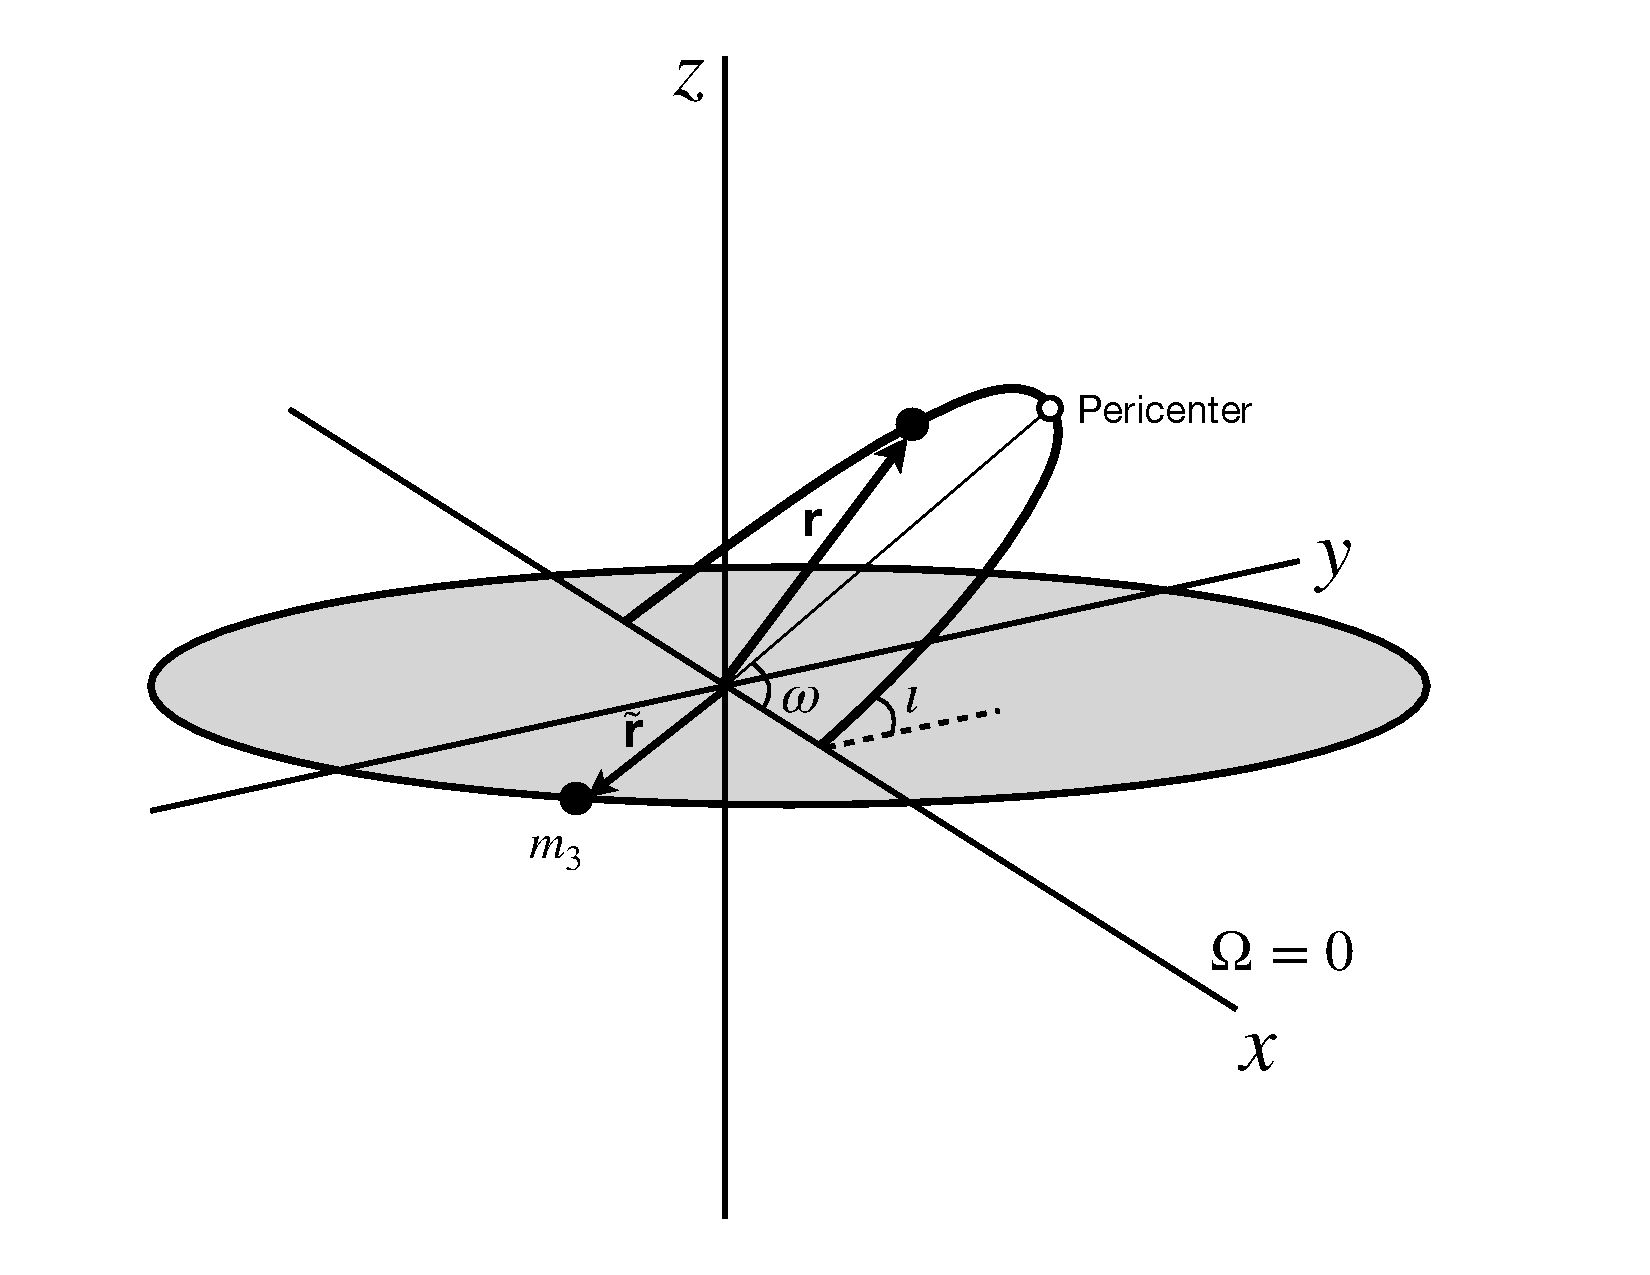
\includegraphics[width=0.6\linewidth]{KozaiLidovSetup}
\caption[Setup for the Kozai-Lidov Effect.]
{\label{fig:KozaiLidovSetup} The three-body system to analyze the Kozai-Lidov effect. We set the fundamental frame such that the orbit of the perturbing body lies in the $xy$-plane and such that the longitude of the ascending node of the 2-body system is $\Omega =0$.}
\end{figure}

We will assume that the perturbing body moves in a circular orbit, defining the normal vector 
\begin{equation}
\tilde{n} = \cos \tilde{f} \textbf{e}_x + \sin \tilde{f} \textbf{e}_y.	
\end{equation}

Using these vectors, we obtain the components of the perturbing force (\ref{eq:PerturbingForceComponentsApprox}) as
\begin{subequations}
 \begin{align}
 \mathcal{S} = &-\frac{Gm_3 r}{\tilde{r}^3} \left[ 1 - 3 \cos^2 \tilde{f} \cos^2 (f+\omega) - 3 \cos^2 \iota \sin^2 \tilde{f} \sin^2 (f+\omega) \right. \notag \\
 &\left. -6 \cos \iota \sin \tilde{f} \cos \tilde{f} \sin (f+\omega) \cos (f+\omega) \right]\\
 \mathcal{T} = &\frac{Gm_3 r}{\tilde{r}^3} \left[ \left( \cos^2 \iota \sin^2 \tilde{f} - \cos^2 \tilde{f} \right) \sin (f+\omega) \cos (f+\omega) \right. \notag \\
 &\left. - \cos \iota \sin \tilde{f} \cos \tilde{f} \left( \sin^2 (f+\omega) -\cos^2 (f+\omega) \right) \right]\\
 \mathcal{W} = &-\frac{Gm_3 r}{\tilde{r}^3} \sin \iota \sin \tilde{f} \left[ \cos \tilde{f} \cos(f+\omega) + \cos \iota \sin \tilde{f} \sin (f+\omega) \right] .
 \end{align}
 \end{subequations} 

By replacing these relations in \ref{eq:OsculatingOrbitalElementsinf}), we obtain a set of differential equations to obtain the changes in the orbital elements. Averaging over the position of the perturbing body,
\begin{equation}
\left\langle \vartheta (\tilde{f} ) \right\rangle = \frac{1}{2 \pi} \int_0^{2\pi} \vartheta (\tilde{f} )  d\tilde{f} ,
\end{equation}
and integrating with respect to $f$ over one period, we obtain the variation of the orbital elements as
\begin{subequations}\label{eq:Kozai-LidovOrbitalElements}
\begin{align}
\left\langle \Delta a \right\rangle &= 0 \\ 
\left\langle \Delta e \right\rangle &= \frac{15 \pi}{2} \frac{m_3}{M} \left( \frac{a}{\tilde{r}}\right)^3 e \sqrt{1-e^2}  \sin^2 \iota \sin \omega \cos \omega \\
\left\langle \Delta \iota \right\rangle &= -\frac{15\pi}{2} \frac{m_3}{M} \left( \frac{a}{\tilde{r}}\right)^3 \frac{e^2}{\sqrt{1-e^2}} \sin \iota \cos \iota \sin \omega \cos \omega \\
\left\langle  \Delta \Omega \right\rangle &= \frac{3\pi}{2} \frac{m_3}{M} \left( \frac{a}{\tilde{r}}\right)^3  \frac{ \cos \iota}{\sqrt{1-e^2}} \left( 5e^2 \cos^2 \omega - 4e^2 -1 \right) \\ 
\left\langle  \Delta \omega \right\rangle &=  \frac{3 \pi}{2} \frac{m_3}{M} \left( \frac{a}{\tilde{r}}\right)^3   \frac{1}{\sqrt{1-e^2}} \left[  5\cos^2 \omega (1-e^2-\cos^2 \iota)- (3(1-e^2) - 5\cos^2 \iota ) \right] \\
\left\langle  \Delta p \right\rangle &= -15 \pi \frac{m_3}{M} \left( \frac{a}{\tilde{r}}\right)^3 a e^2  \sqrt{1-e^2} \sin^2 \iota \sin \omega \cos \omega.
\end{align}
\end{subequations}

\textbf{Angular Momentum Conservation}

From the Figure \ref{fig:KozaiLidovSetup} , it can be seen that the $z$-component of the total angular momentum of the system can be written as
\begin{equation}
\boldsymbol{\ell} ^z_{total} = \boldsymbol{\ell}^z + \tilde{\boldsymbol{\ell}}^z
\end{equation}
where $\boldsymbol{\ell}$ is the angular momentum of the binary system and $\tilde{\boldsymbol{\ell}}$ is the angular momentum associated with the orbital motion of the third body. Assuming that the objects $m_1$ and $m_2$ don't affect the motion of the third body, we consider that $\tilde{\boldsymbol{\ell}}$ is conserved. Hence, the question arising is about the conservation of the component $\boldsymbol{\ell}^z$ of the binary system, which is
\begin{equation}
\ell^z = \boldsymbol{\ell} \cdot \textbf{e}_z = \sqrt{GMa(1-e^2)} \cos \iota.
\end{equation}

From this relation it is possible to obtain the change in this quantity, averaged over one orbit of the third body, as
\begin{equation}
\frac{\left\langle \Delta \ell^z \right\rangle }{\sqrt{GM}}= \frac{(1-e^2)\left\langle \Delta a \right\rangle - 2ae \left\langle \Delta e \right\rangle}{2 \sqrt{a(1-e^2)} }\cos \iota - \sqrt{a(1-e^2)} \sin \iota  \left\langle \Delta \iota \right\rangle .
\end{equation}

Using the results (\ref{eq:Kozai-LidovOrbitalElements}), we confirm immediately the conservation law $\left\langle \Delta \ell^z \right\rangle=0$. Since $\left\langle \Delta a \right\rangle=0$, the conservation statement is equivalent to the relation
\begin{equation}
\frac{e}{1-e^2} \left\langle \Delta e \right\rangle + \tan \iota \left\langle \Delta \iota \right\rangle = 0.
\end{equation}

This result is known as the \textit{Kozai-Lidov effect} and implies an exchange between eccentricity and inclination of the orbit. In order to analyze this effect, consider the factor $\left[  5\cos^2 \omega (1-e^2-\cos^2 \iota)- (3(1-e^2) - 5\cos^2 \iota ) \right]$ in the equation for $\left\langle \Delta \omega \right\rangle$. From it, we find a critical value $\omega_c$ for which $\left\langle \Delta \omega \right\rangle= 0$,
\begin{equation}
\cos^2 \omega_c = \frac{3(1-e^2) - 5\cos^2 \iota }{5 (1-e^2-\cos^2 \iota)}.
\end{equation}

If $\cos^2 \iota > \frac{3}{5}(1-e^2)$, i.e. for small initial inclination angles, the critical value $\omega_c$ doesn't exists and therefore, the argument of the pericenter $\omega$ increases monotonically while  eccentricity and inclination present a periodic exchange, as seen in Figure \ref{fig:KozaiLidovEffect1}. In this case, the longitude of the ascending node $\Omega$ also increases monotonically. 

\begin{figure}[h]
\centering
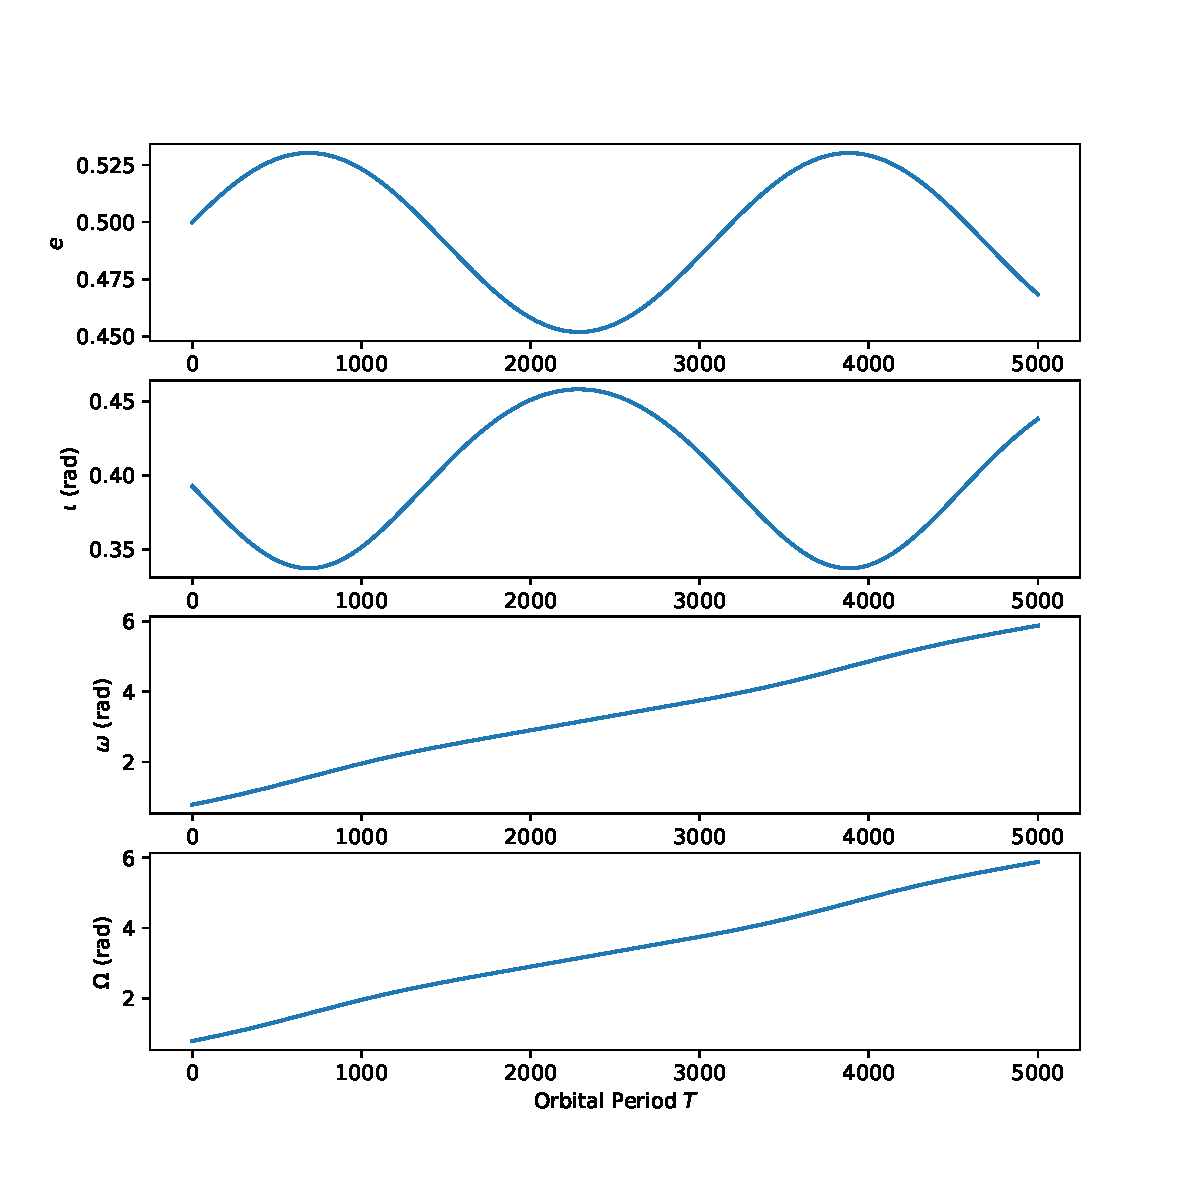
\includegraphics[width=0.6\linewidth]{KozaiLidov}
\caption[Kozai-Lidov Effect.]
{\label{fig:KozaiLidovEffect1} This plot shows the Kozai-Lidov effect as a periodic exchange between eccentricity and inclination of the orbit. This oscillatory behavior is obtained from equations (\ref{eq:Kozai-LidovOrbitalElements}) and occurs when the inclination angle of the orbit is small (see text for details). We also include the advance of the pericenter and the shift in the longitude of he ascending node. We use the values $m_3 = 0.1 M$ and $a=0.1 \tilde{r}$, together with the initial values $e_0 = 0.5$, $\omega_0 = \frac{\pi}{4}$, $\iota_0 = \frac{\pi}{8}$ and $\Omega_0 = 0$. }
\end{figure}

On the other hand, a high  initial inclination angle, such that $\cos^2 \iota < \frac{3}{5}(1-e^2)$ gives a real value for the critical value $\omega_c$. Figure \ref{fig:KozaiLidovEffect2} shows that in this case the argument of the pericenter increases until it reaches the critical value and, since this gives $\left\langle \Delta \omega \right\rangle= 0$, the evolution of $\omega$ stops. This also stops the evolution of $e$, $\iota$ and $\Omega$ so that there is no periodical behavior in the orbital parameters but they reach a stable equilibrium state.

\begin{figure}[h]
\centering
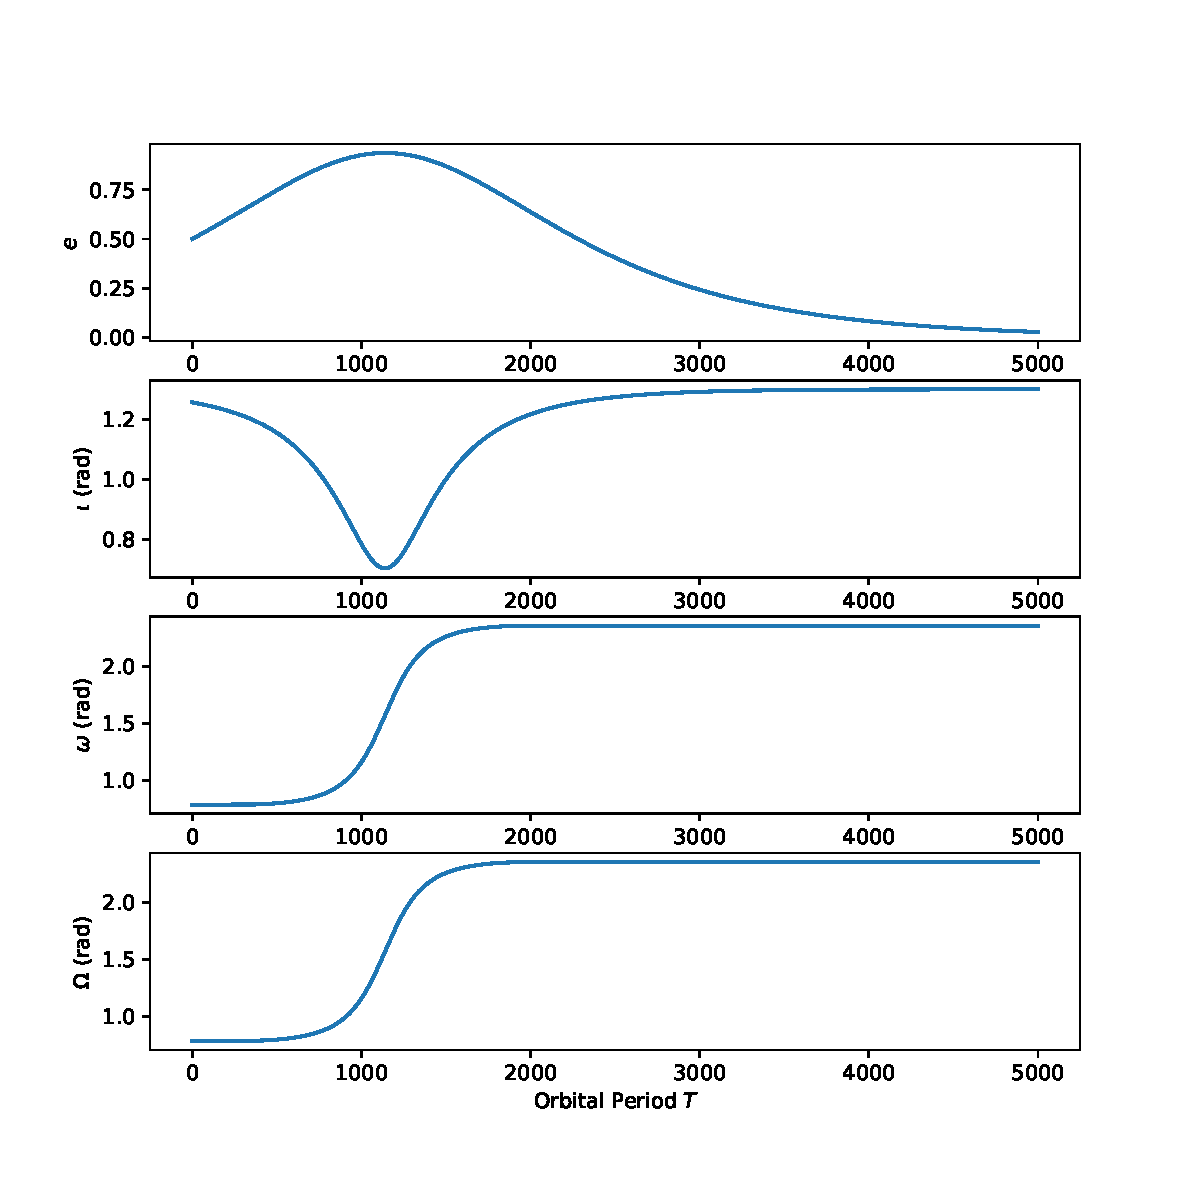
\includegraphics[width=0.6\linewidth]{KozaiLidovCritical}
\caption[Critical Kozai-Lidov Effect.]
{\label{fig:KozaiLidovEffect2} When the orbit has a high initial inclination angle, the Kozai-Lidov effect doesn't have an oscillatory exchange. In this case, the argument of the pericenter approaches a critical value for which $\left\langle \Delta \omega \right\rangle = 0$ and therefore the perihlion shift stops as well as the changes in eccentricity and inclination(see text for details). We use the values $m_3 = 0.1 M$ and $a=0.1 \tilde{r}$, together with the initial values $e_0 = 0.5$, $\omega_0 = \frac{\pi}{4}$, $\iota_0 = \frac{2\pi}{5}$ and $\Omega_0 = 0$. }
\end{figure}

% Perturbation in terms of a Perturbing Lagrangian.
%\section{Lagrange Planetary Equations}
%Although equations (\ref{eq:OsculatingOrbitalElements}) are valid for any perturbation, there is an interesting form of writing those equations when the perturbing force can be obtained from a disturbing Lagrangian. Suppose that the complete Lagrangian of the perturbed system can be written as
%\begin{equation}
%L = \frac{1}{2} \mu \dot{\textbf{r}}^2 + \frac{GM\mu}{r} + \mu R
%\end{equation}
%where $R=R(\textbf{r}, \dot{\textbf{r}} ; t)$ is a function that produces the perturbing term in the equations of motion through the relation
%\begin{equation}
%\delta \textbf{A} = \frac{\partial R}{\partial \textbf{r}} - \frac{d}{dt} \left( \frac{\partial R}{\partial \dot{\textbf{r}}} \right).
%\end{equation}
%
%The canonical conjugate momenta are defined as usual,
%\begin{equation}
%\textbf{p} = \frac{\partial L}{\partial \dot{\textbf{r}}} = \mu \dot{\textbf{r}} + \mu \frac{\partial R}{\partial \dot{\textbf{r}}},
%\end{equation}
%and therefore, the Hamiltonian of the system is
%\begin{equation}
%H = \frac{1}{2\mu} \textbf{p}^2 - \frac{GM\mu}{r} - \mu V
%\end{equation}
%where we defined the term
%\begin{equation}
%V = \mu R + \frac{1}{2} \mu \left( \frac{\partial R}{\partial \dot{\textbf{r}}} \right)^2
%\end{equation}

%\section{Problems}
%\begin{enumerate}
%\item The Jupiter 
%\end{enumerate}


